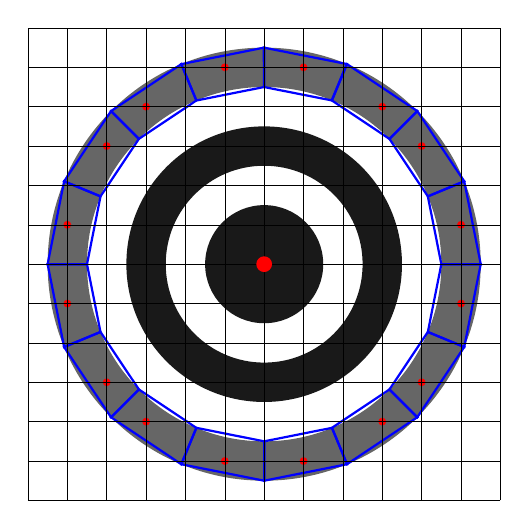
\begin{tikzpicture}[scale=0.5]
	\fill[black!90!white] (0,0) circle [radius=1.5];
	\fill[black!90!white, even odd rule] (0,0) circle[radius=2.5] circle[radius=3.5];
	\fill[black!60!white, even odd rule] (0,0) circle[radius=4.5] circle[radius=5.5];
	
	\fill[red] (5,1) circle [radius=0.1]; 
	\fill[red] (4,3) circle [radius=0.1]; 
	\fill[red] (3,4) circle [radius=0.1]; 
	\fill[red] (1,5) circle [radius=0.1]; 
	\fill[red] (-1,5) circle [radius=0.1]; 
	\fill[red] (-3,4) circle [radius=0.1]; 
	\fill[red] (-4,3) circle [radius=0.1]; 
	\fill[red] (-5,1) circle [radius=0.1]; 
	\fill[red] (-5,-1) circle [radius=0.1]; 
	\fill[red] (-4,-3) circle [radius=0.1]; 
	\fill[red] (-3,-4) circle [radius=0.1]; 
	\fill[red] (-1,-5) circle [radius=0.1]; 
	\fill[red] (1,-5) circle [radius=0.1]; 
	\fill[red] (3,-4) circle [radius=0.1]; 
	\fill[red] (4,-3) circle [radius=0.1]; 
	\fill[red] (5,-1) circle [radius=0.1];  

	\foreach \angle in {0, 22.5, 45, 67.590, 90, 112.5, 135, 157.5, 180, 202.5, 225, 247.5, 270, 292.5, 315, 337.5} 
	\draw[blue, thick] (\angle:4.5) -- (\angle:5.5) -- (\angle+22.5:5.5) -- (\angle+22.5:4.5) -- cycle;

	\draw[very thin] (-6, -6) grid (6, 6);
	\fill[red] (0,0) circle[radius=0.2];
\end{tikzpicture}